\section{Reducing The Branching Factor}
The branching factor associated with each tile on the perimeter of an empty room (in an 8-connected 
grid map) is dependent on the dimensions of the room.
Consider an empty room of width $w$ and height $h$ where $w > h$.
After adding all non-dominated macro edges to the room, each tile is incident with at least $h$ macro edges and up to $2h-1$ 
depending on its positon on the perimeter.
Further, each tile is adjacent with 2 other tiles from the perimeter of the same room and up to 3 tiles from an adjacent room.
Thus the total branching factor for each tile is at least $h + 2$ and can be as high
as $2h + 4$.
Generally speaking, a large branching factor is undesirable for two reasons:
(i) invididual node expansion operations take longer and (ii) additional neighbours usually 
add more branches to the search tree and make it more difficult to reach the goal.
\par
In this section we discuss two novel optimality preserving methods for reducing branching factor. 
The first is an offline perimeter reduction method while the second is an online optimisation which speeds up 
node expansion when searching along the perimeter of an empty room.
We will discuss both methods in the context of 8-connected grid maps.
Analogous algorithms, suitable to 4-connected grid maps, are easily derived.
\par \noindent \newline
\textbf{Perimeter Reduction:}
We observe that in many cases there are tiles on the perimeter of an empty room which have no neighbours from any 
adjacent room. 
These tiles represent intermediate locations between entry and exit points that lead into and out of each empty room.
To speed up search we propose pruning from the perimeter of each room all such nodes.
To preserve optimality, we will connect the neighbours of each pruned node directly to each other.
The weight of each new edge is therefore equal to the octile distance between the two neighbours.
Figure \ref{fig-reduction} shows an example.
This is a very simple optimisation but as we will see, it can have a dramatic effect on the average performance of
A* on certain types of maps.
\par \noindent \newline
\textbf{Faster Node Expansion:} 
We propose the following online symmetry elimination tehcnique:
\begin{enumerate}
\item{}
\end{enumerate}

\begin{figure}[tb]
       \begin{center}
                       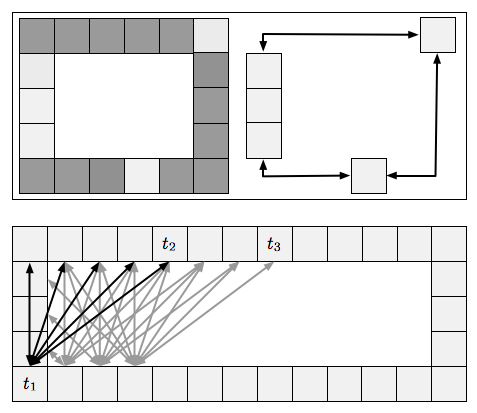
\includegraphics[scale=0.5, trim = 10mm 10mm 10mm 0mm]{diagrams/branching.png}
       \end{center}
	\vspace{-3pt}
       \caption{(Top) An empty room. Dark grey tiles have no neighbours from any adjacent room. 
We prune these nodes and connect their neighbours directly (not all macro edges shown).
		(Bottom) A path enters an empty room at tile $t1$ and exits at tile $t2$. Notice that once
$t1$ is expanded every path to $t2$ is dominated by a path that starts at $t1$ and mentions one of its macro edges.
}
       \label{fig-macroedges}
\end{figure}
